\section{Background} \label{background}

The Dragonfly relocatable lander, illustrated in Figure~\ref{fig:dragonfly}, is equipped with two \acp{IMU}, two pressure sensors, one lidar, and one \ac{NavCam}. The sensor rates and measurement types are listed in Table~\ref{tab:sensor}. Further details of the baseline sensor specifications are captured in Table~\ref{tab:sim_setup} of the \nameref{results} section.

\begin{minipage}{\textwidth}
  \begin{minipage}[b]{0.49\textwidth}
    \centering
    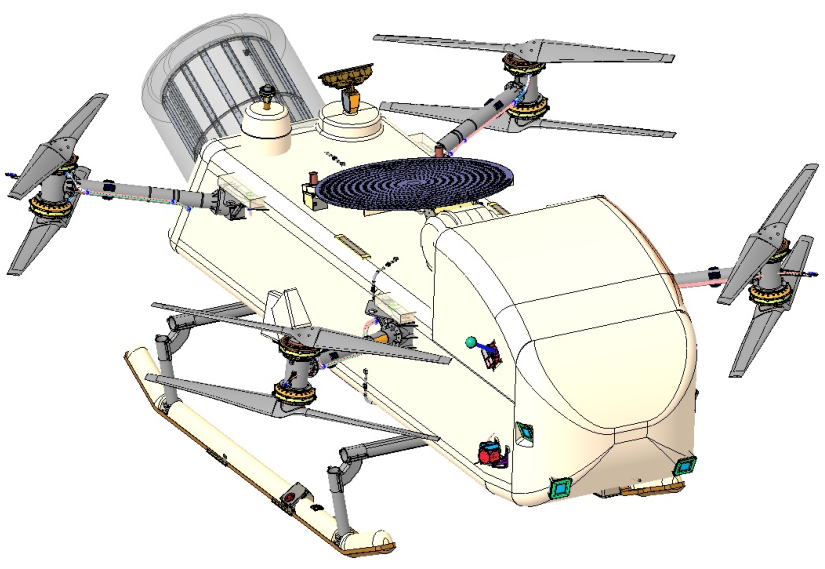
\includegraphics[width=3in]{content/figures/lander_selective_redundancy.pdf}
    \captionof{figure}{Dragonfly relocatable rotorcraft}
    \label{fig:dragonfly}
  \end{minipage}
  \hfill
  \begin{minipage}[b]{0.49\textwidth}
  	\fontsize{9}{8}\selectfont
    \centering
   \begin{tabular}{| c | c | c |} % Column formatting, 
      \hline 
      Sensor & Rate (Hz) & Measurement \\
      \hline 
     IMU (x2) & 200 & $\Delta$V,$\Delta\theta$ \\ 
      Pressure (x2) & 10 & Absolute pressure\\
     Lidar & 5-10\tablefootnote{The lidar runs at higher rates during hazard detection scans, but only a subset of data is used by the nav filter} & X,Y,Z point \\
     NavCam/ETS & 1 & Position displacement \\      \hline
   \end{tabular}
      \captionof{table}{Dragonfly sensor suite}
      \label{tab:sensor}
      \vspace*{0.6in}
    \end{minipage}
\end{minipage}

\noindent The NavCam images are processed by the \ac{ETS} module, which correlates two images to generate a lateral position displacement measurement for the nav filter.\cite{witte2019no, jenkins2022} The two \ac{NavCam} images are referred to as the $\it{current}$ image and $\it{reference}$ image. The current image is always the most recent image captured by the \ac{NavCam}, while the reference image used for correlation can be one of several types as listed in Table~\ref{tab:ets_modalities}. For recent reference images still in view of the current image, the position and velocity errors in the nav filter are highly correlated.  This position displacement measurement provides observability into velocity. Online breadcrumbs are periodically saved when one of two thresholds are crossed. The first threshold defines the maximum lateral distance scaled by the altitude from the last breadcrumb location. This threshold can also be viewed as a maximum angular or pixel offset in the camera. The second threshold type is based on a maximum scale variation defined as a maximum vertical distance over the altitude from the last breadcrumb. When an online breadcrumb is saved, the position, attitude, height \ac{AGL}, and covariance are saved in a database along with the image to allow the vehicle to retrace the path on the same flight. Following a flight, a subset of online breadcrumbs are converted into historic breadcrumbs for the next flight, which allows the vehicle to retrace segments of the previous flight. Details of this process are covered in the \nameref{design} section. The terminal breadcrumb distinction is given to images containing the landing site, where the landing site position relative to the breadcrumb image position is known to high accuracy. 
\begin{table}[htbp]
	\fontsize{10}{10}\selectfont
    \caption{ETS Measurement Modalities}
   \label{tab:ets_modalities}
        \centering 
   \begin{tabular}{|c c|} % Column formatting, 
      \hline 
      Modality & Reference Image  \\
      \hline 
      Velocimetry & Still in NavCam FOV \\
      Online Breadcrumb & Captured earlier on current flight  \\
      Historic Breadcrumb & Captured during a previous flight \\
      Terminal Breadcrumb & Captured on current/previous flight and contains landing site  \\
      \hline
   \end{tabular}
\end{table}
Figure~\ref{fig:breadcrumbs} illustrates the primary Mobility flight types including a Scout, where the vehicle scouts a new candidate landing zone then returns to the take-off site, and a Leapfrog, where the vehicle scouts a new candidate landing zone then lands at a site that was previously scouted.
\begin{figure}[htbp]
	\centering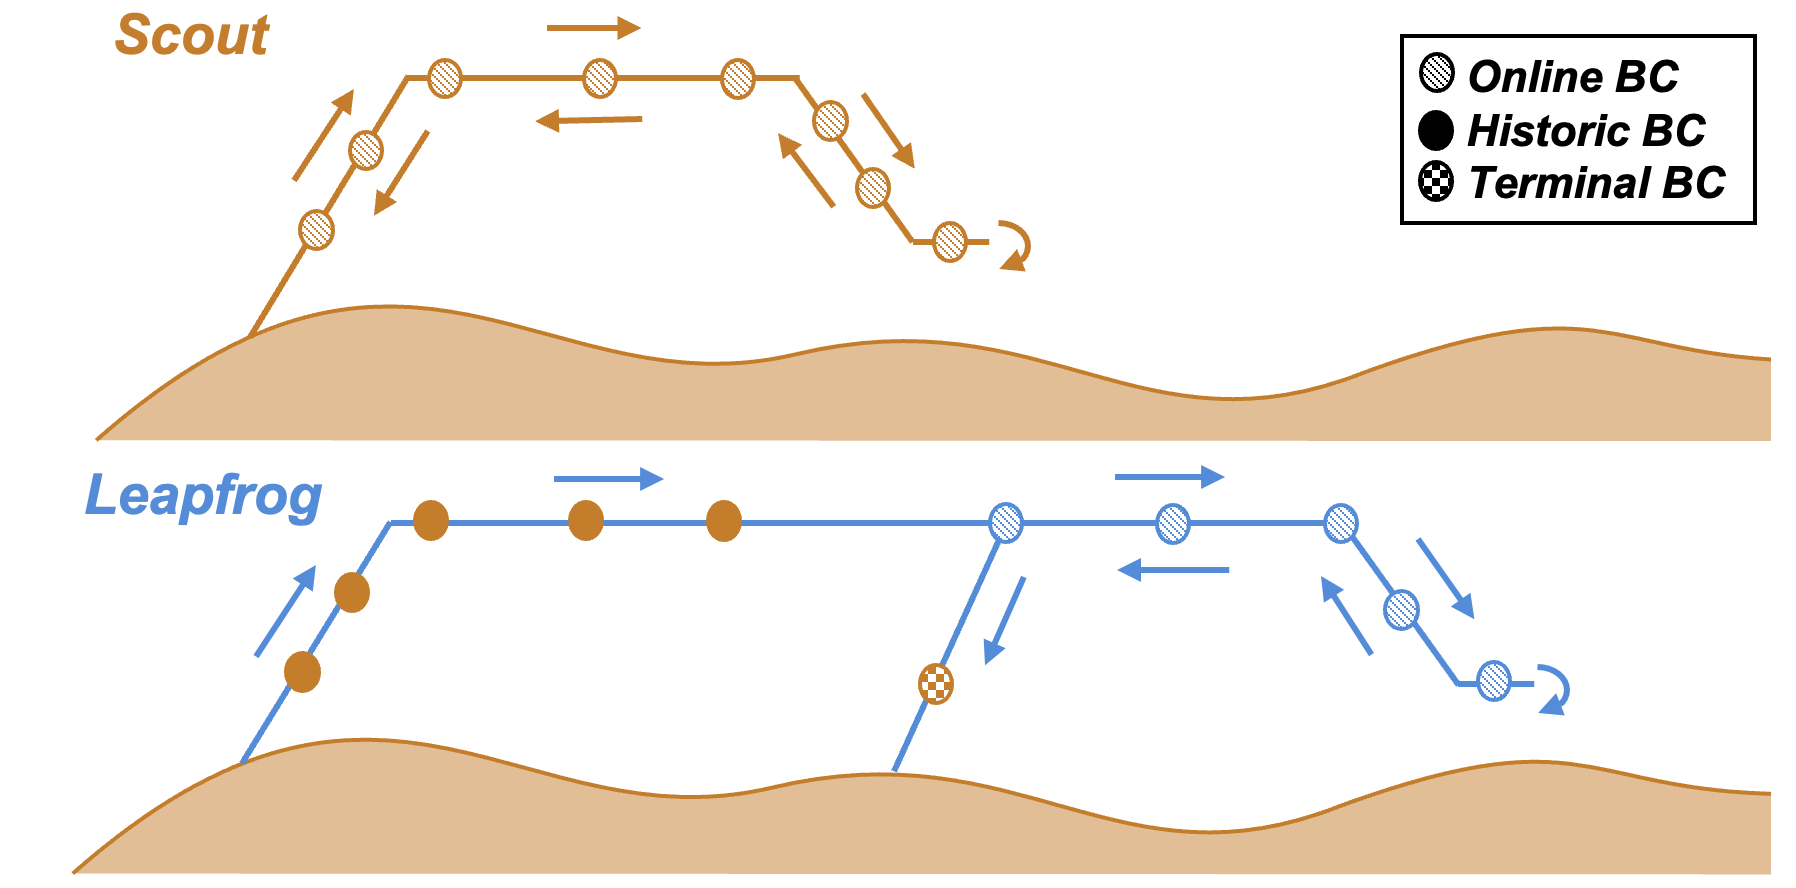
\includegraphics[width=6in]{content/figures/breadcrumbs.png}
	\caption{Mobility CONOPS and flight types}
	\label{fig:breadcrumbs}
\end{figure}
\subsection{Coordinate Frames}

Several coordinate frames are utilized by the navigation formulation. The \ac{TCI} frame is the inertial reference frame for Titan, similar to Earth-Centered Inertial.\cite{Archinal} The \ac{TCTF} is the rotating frame, with the Z-axis aligned with Titan rotation. The \ac{NED} frame is a local tangent frame where north points to the Titan spin vector (i.e. true North), down is aligned with plumb bob gravity, and east completes the right hand triad. The NED frame rotates with Titan, with the origin at the take-off position. The primary navigation frame is the \ac{TOF}, where the origin is also at the take-off position, but the frame is aligned with the $\it{estimated}$ north, east, and down directions. The TOF contains errors with respect to NED due to initial attitude errors, but by definition, does not include absolute position errors due to absolute heading error. This nuance is further discussed in the \nameref{design} section. The Dragonfly body frame uses the \ac{FRD} convention. Finally, there are instrument frames for both \acp{IMU}, the lidar, and \ac{NavCam}. 